\documentclass{beamer} 
\usepackage{beamerthemeshadow}
\usepackage[latin1]{inputenc}
\usepackage[brazil]{babel}
\usepackage{graphicx}
\usepackage{pgfpages}
\usepackage{listings}
\title[]{Uso de padr\~ao AMQP para transporte de mensagens entre atores remotos} 
\author{Thadeu de Russo e Carmo \\ \texttt{thadeurc@ime.usp.br}}
\institute{Orientador: Prof. Dr. Francisco da Rocha Reverbel\\ Instituto de Matem\'atica e Estat\'istica \\ Universidade de S\~ao Paulo}
\date{Abril, 2012}
\setbeameroption{show notes on second screen=left} 
\begin{document}
\frame{\titlepage}
\section{Introdu\c{c}\~ao} 
\subsection{Motiva\c{c}\~ao}
\setbeamertemplate{footline}[page number]
\frame{\frametitle{Motiva��o}
	\note{Apenas comentar o que esta no slide.}
    	\only<1>{
     		Explorar a potencial sinergia entre duas classes de sistemas de \textit{software}:
 		\begin{enumerate}
 			\item Sistemas corporativos: composta de sistemas de \textit{middleware} orientados a mensagens e 
				\textit{message brokers}
			\item Programas concorrentes: composta pelas implementa\c{c}\~oes do modelo de atores
 		\end{enumerate}
	}
}

\frame{
\frametitle{Motiva\c{c}\~ao -- Sistemas corporativos}
	\only<1>{
 		\note{
 			\begin{itemize}
 				\item Comentar sobre o nao vinculo de produtor e consumidor com cliente (usuario de um servico)
 			         e servidor (provedor de um servico) -- cliente/servidor eh baseado na semantica das
				mensagens
				\item Baixo acoplamento e interoperabilidade
				\item filas transacionais (abstracao -- persistente) provem a garantia de entrega
 			\end{itemize}
		}
		\begin{itemize}
			\item \textit{Middlewares} orientados a mensagem (MOMs) trabalham com troca ass\'incrona de mensagens
			\item Formam base para simplificar o desenvolvimento de sistemas
			\item Possuem suporte e mecanismos para gerenciamento robusto de erros e garantia de entrega de mensagens	
			\item S\~ao frequentemente apresentados como tecnologia que pode mudar a maneira como sistemas distribu\'idos
			s\~ao constru\'idos [Alonso et al 2004]
		\end{itemize}
	}
	\only<2>{
 		\note{ 
 			\begin{itemize}
 				\item o que era no nivel da aplicacao foi para o nivel de configuracao (e.g.: MDB
				declara no seu registro as mensagens que vao filtrar)
				\item regras de negocio para roteamento -- WSMB 6.1
			\end{itemize}
		}
 		\begin{itemize}
			\item MOMs s\~ao um tanto quanto inflex\'iveis em rela\c{c}\~ao a filtragem e roteamento de mensagens
			\item \textit{Message brokers} s\~ao descendentes diretos dos MOMs e endere\c{c}am essas limita\c{c}\~oes
		\end{itemize}
	}
	\only<3>{
 		\note{
 			\begin{itemize}
	 			\item Lembrar dos altos custos altos -- MQSeries
			\end{itemize}
		}
 		Os protocolos usados por \textit{message brokers} variam de produto para produto. Algumas abordagens existentes:
 		\begin{itemize}
 			\item A especifica\c{c}\~ao Java \textit{Message Service} (JMS) define uma API padr\~ao para que programas Java possam
			interagir com \textit{message brokers}
 			\item O padr�o \textit{Advanced Message Queuing Protocol} (AMQP) \'e uma proposta
 			recente de padroniza\c{c}\~ao de protocolo para \textit{message brokers}
 		\end{itemize}
	}
}
\frame{
\frametitle{Motiva\c{c}\~ao -- Programas concorrentes}
	\only<1>{
		\note{
 			\begin{itemize}
	 			\item The free lunch is over -- limites fisicos
				\item locks -- nao compoem de modo seguro - lembrar que so podemos pegar um lock por vez
			\end{itemize}
		}

		Processadores \textit{multicore} impactam a maneira que programas s\~ao escritos:
		\begin{itemize}
			\item  Programas precisam ser escritos de maneira concorrente para poder
			usufruir dos ganhos de desempenho dos processadores \textit{multicore} [Sutter 2005]
			
			\item Abordagem convencional com o uso de travas, al\'em de complexa, � limitada e n\~ao permite a
			composi��o das travas de modo seguro [Jones 2007]

			\item A maioria das linguagens de programa\c{c}\~ao n\~ao s\~ao adequadas para a cria\c{c}\~ao de tais
			programas [Sutter \& Larus 2005]
		\end{itemize}
	}
	\only<2>{
 		\note{
 			\begin{itemize}
	 			\item STM compartilha tudo, eh componivel -- programas lineares, mas nao eh bom
				para o caso distribuido
				\item Atores -- nao compartilha nada -- programas nao lineares, mas
				distribui bem - falar da ordem parcial de tempo
			\end{itemize}
		}
		Modelos n\~ao convencionais de programa\c{c}\~ao concorrente:
		\begin{itemize}
			\item \textit{Software Transactional Memory} (STM) -- mecanismo de controle an\'alogo
			\`as transa\c{c}\~oes de bancos de dados
			\item Atores -- troca de mensagem ass\'incrona entre processos 
		\end{itemize}
	}
}
\frame{
\frametitle{Motiva\c{c}\~ao}
	\only<1>{
 		\note{
 			\begin{itemize}
	 			\item nao ha cliente servidor
				\item troca assincrona
				\item garantia de entrega de mensagens
			\end{itemize}
		}

		Potencial sinergia entre as duas classes:
		\begin{itemize}
			\item Atores em diferentes n\'os em uma rede de computadores podem trocar mensagens entre si
			\item \textit{Message brokers} prov\^em robustez para a troca de mensagens entre entidades em diferentes n\'os de um sistema
		\end{itemize}
	}
}
\frame{
\frametitle{Objetivos}
	Este trabalho teve como objetivos a cria\c{c}\~ao de uma implementa\c{c}\~ao em Scala do modelo de atores que utilize o padr\~ao AMQP
	para o transporte de mensagens entre atores remotos.
}
\subsection{Atores}
\frame{
\frametitle{Atores}
	\only<1>{
 		\note{
 			\begin{itemize}
	 			\item So resumir o slide - comentar do Hewitt e falar que tbm cliente/servidor
				varia de acordo com os a semantica das mensagens.
			\end{itemize}			
		}

		\begin{beamerboxesrounded}{Defini\c{c}\~ao de um Ator [Agha 1986]}
			\'E um agente computacional que possui uma caixa de correio e um comportamento.
			Atores processam assicronamente as mensagens recebidas em suas respectivas caixas de correios. 
			As mensagens recebidas s\~ao mapeadas em uma $3$-tupla consistindo de: 
			\begin{itemize}
				\item Um conjunto finito de mensagens enviadas para outros atores onde o endere\c{c}o \'e conhecido
				(um deles pode ser o pr\'oprio ator que est\'a processando a mensagem)
				\item Um novo comportamento a ser usado no processamento da mensagem seguinte
				\item Um conjunto finito de cria\c{c}\~oes de novos atores
			\end{itemize}
		\end{beamerboxesrounded}
	}
%% ainda nao estou certo de mostrar animado ou fixo
	\only<2>{
 		\begin{figure}[hbtp]
			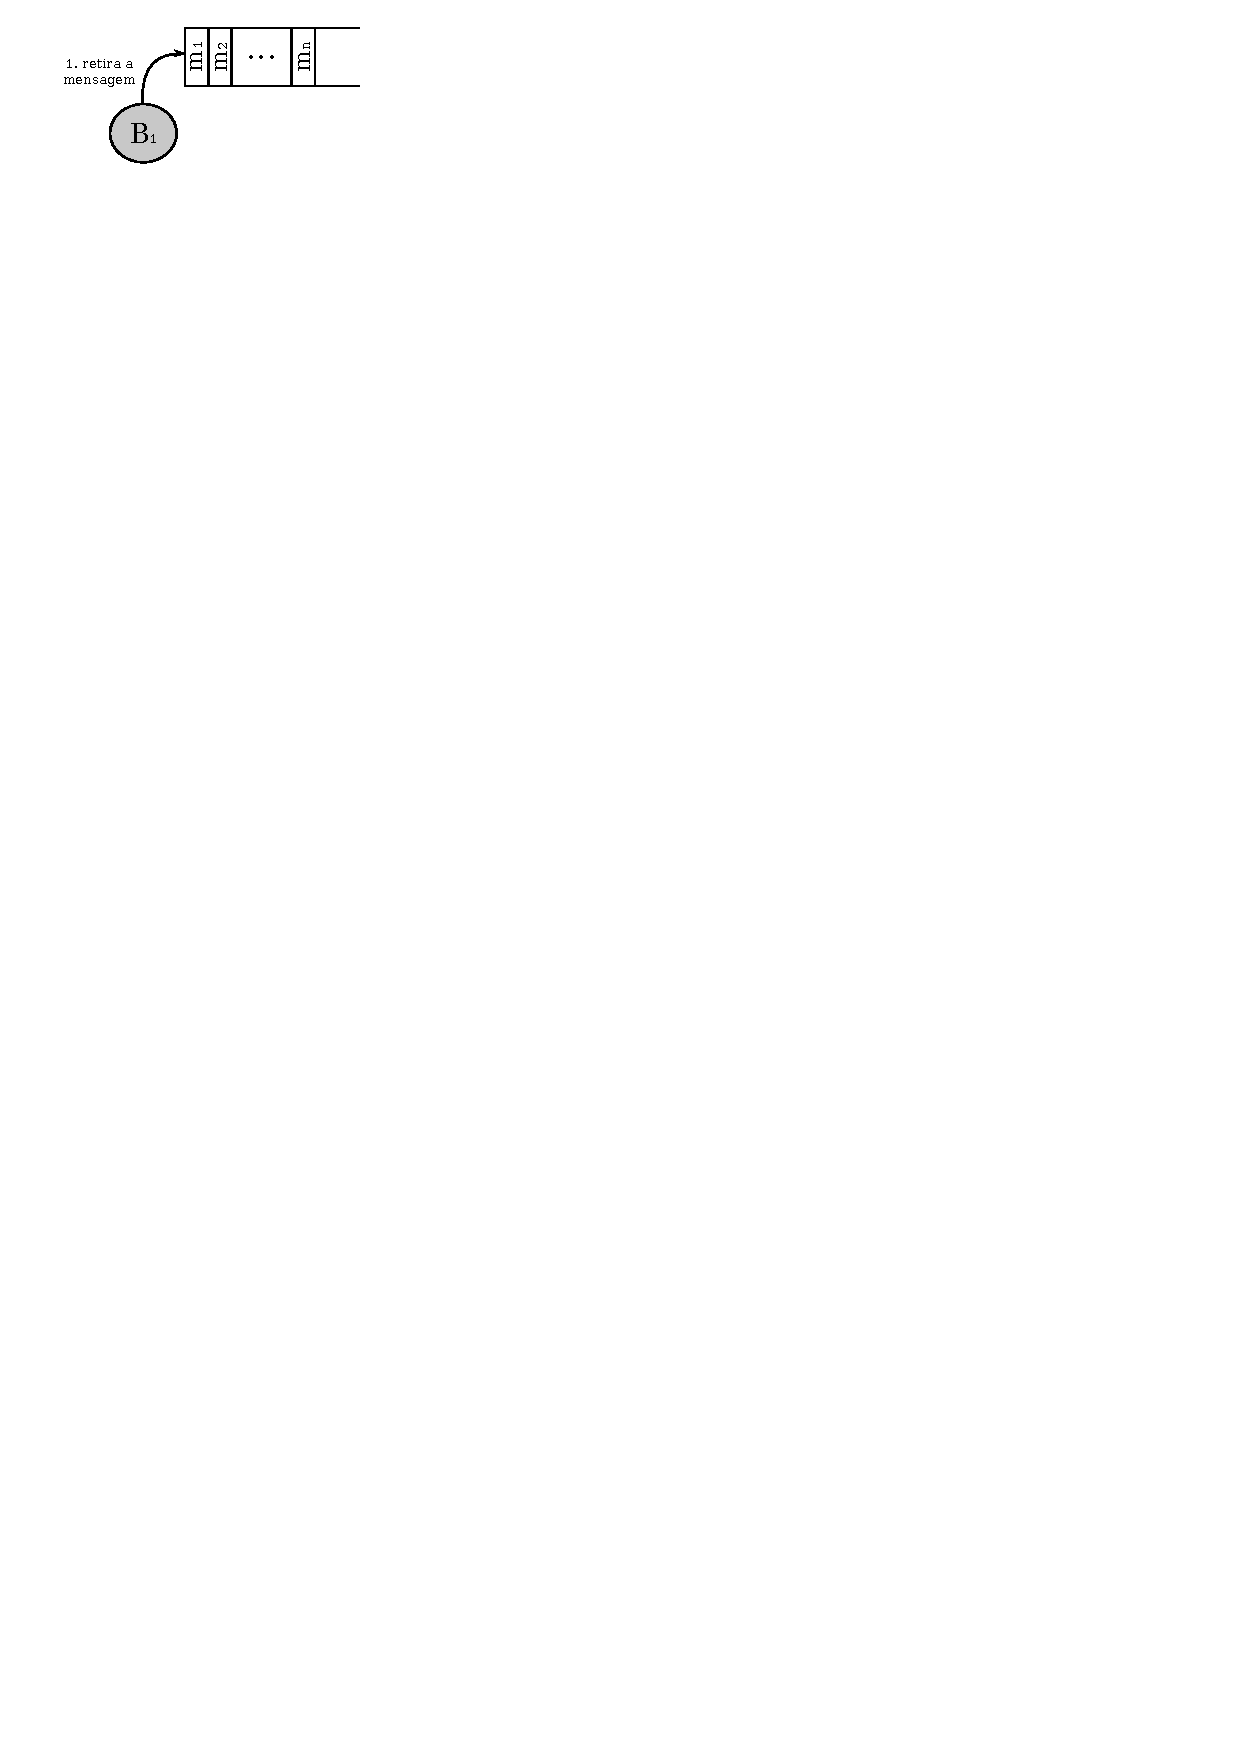
\includegraphics[scale=1.0]{figuras/ator-state-machine0.pdf}
		\end{figure}
 	}
	\only<3>{
 		\begin{figure}[hbtp]
			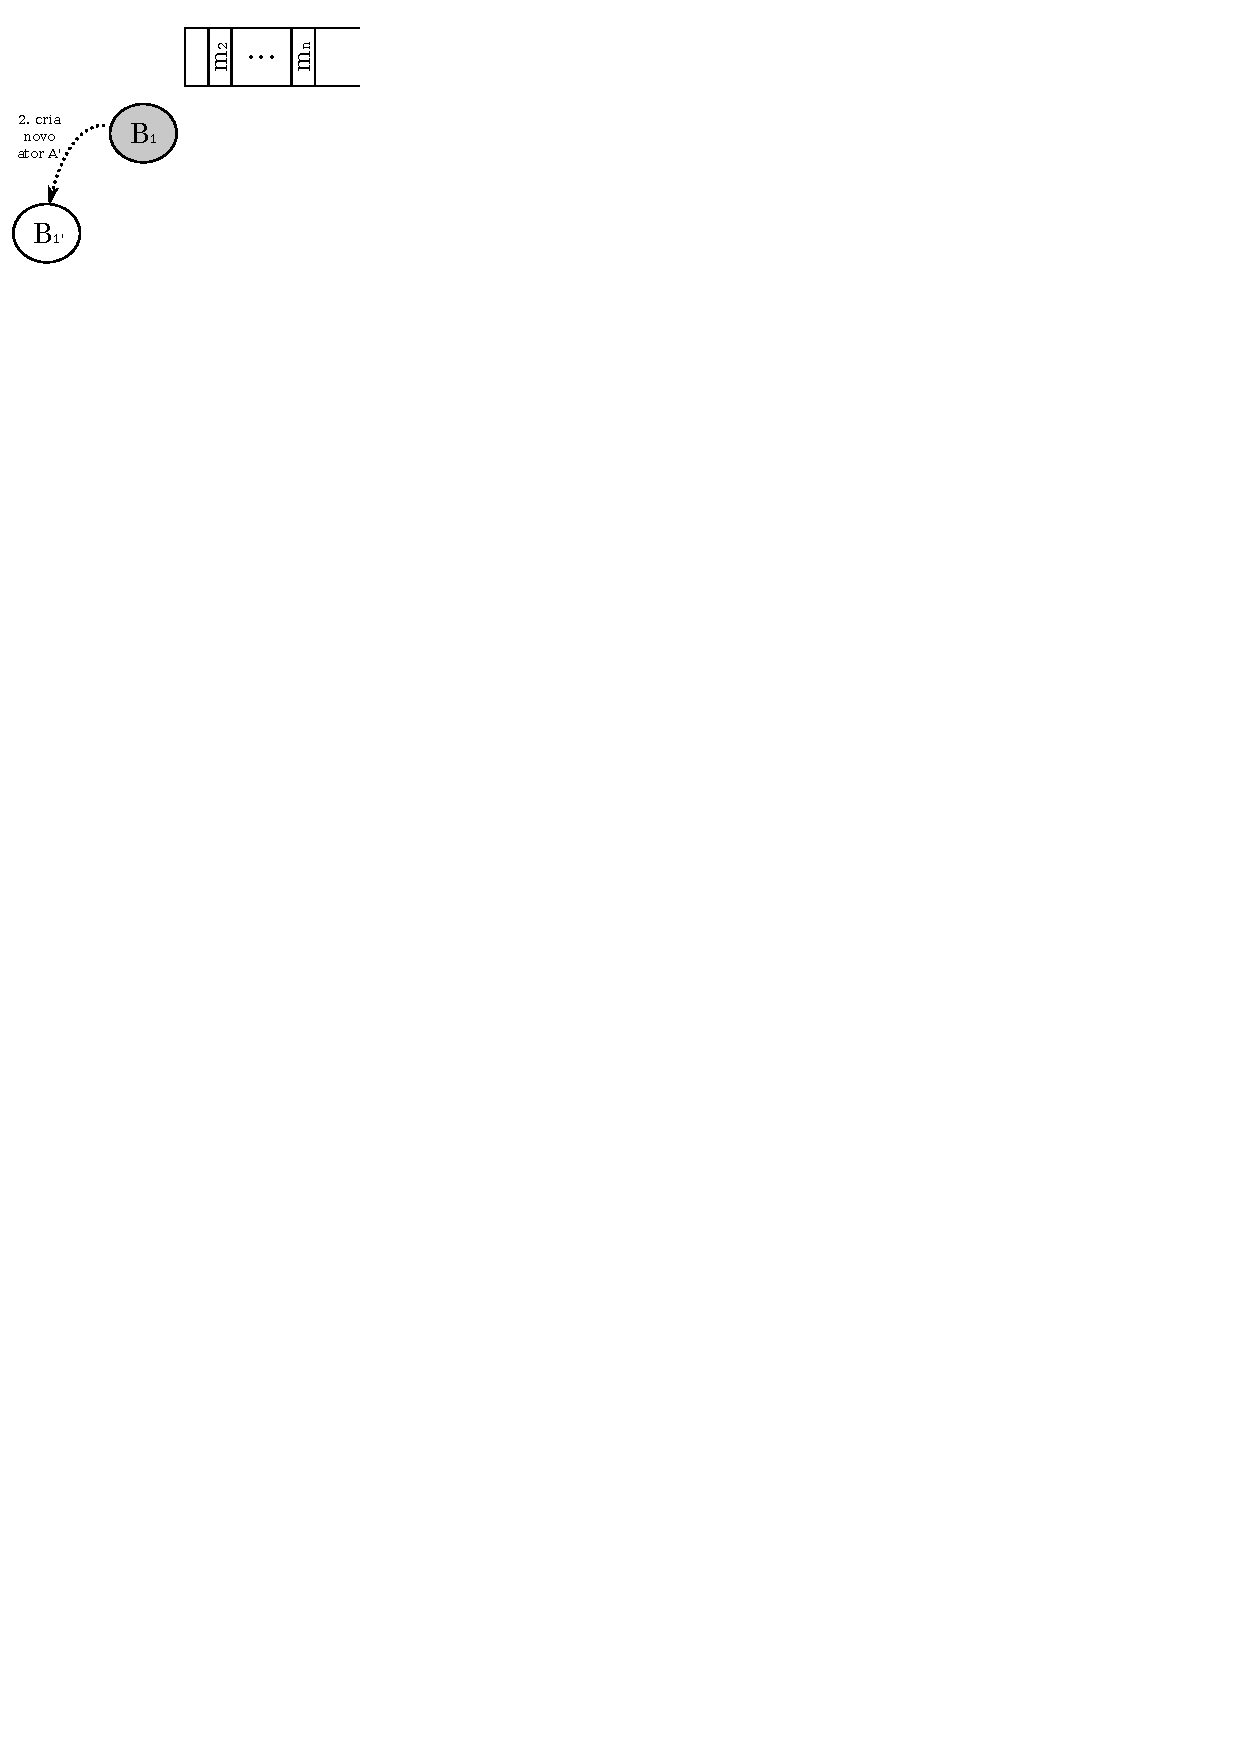
\includegraphics[scale=1.0]{figuras/ator-state-machine1.pdf}
		\end{figure}
 	}	
	\only<4>{
 		\begin{figure}[hbtp]
			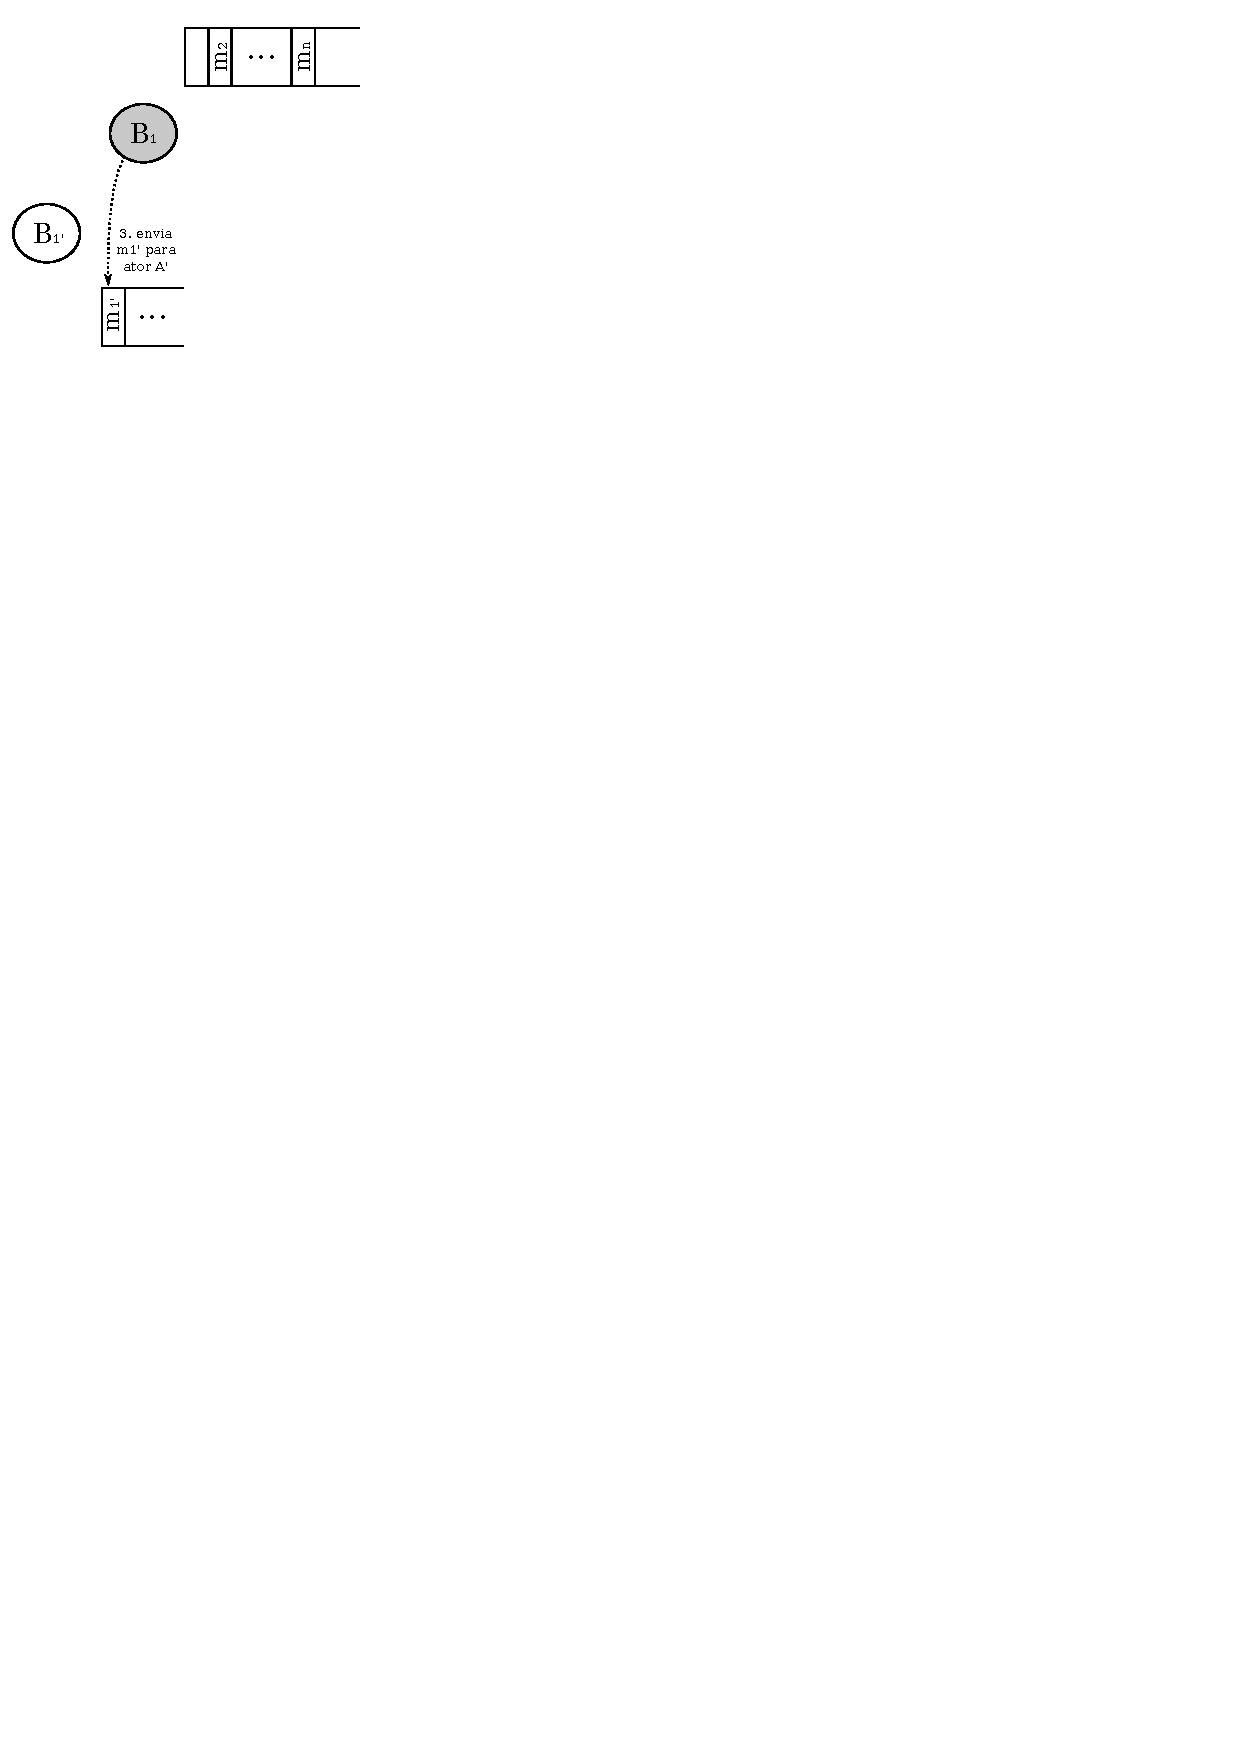
\includegraphics[scale=1.0]{figuras/ator-state-machine3.pdf}
		\end{figure}
 	}
	\only<5>{
 		\begin{figure}[hbtp]
			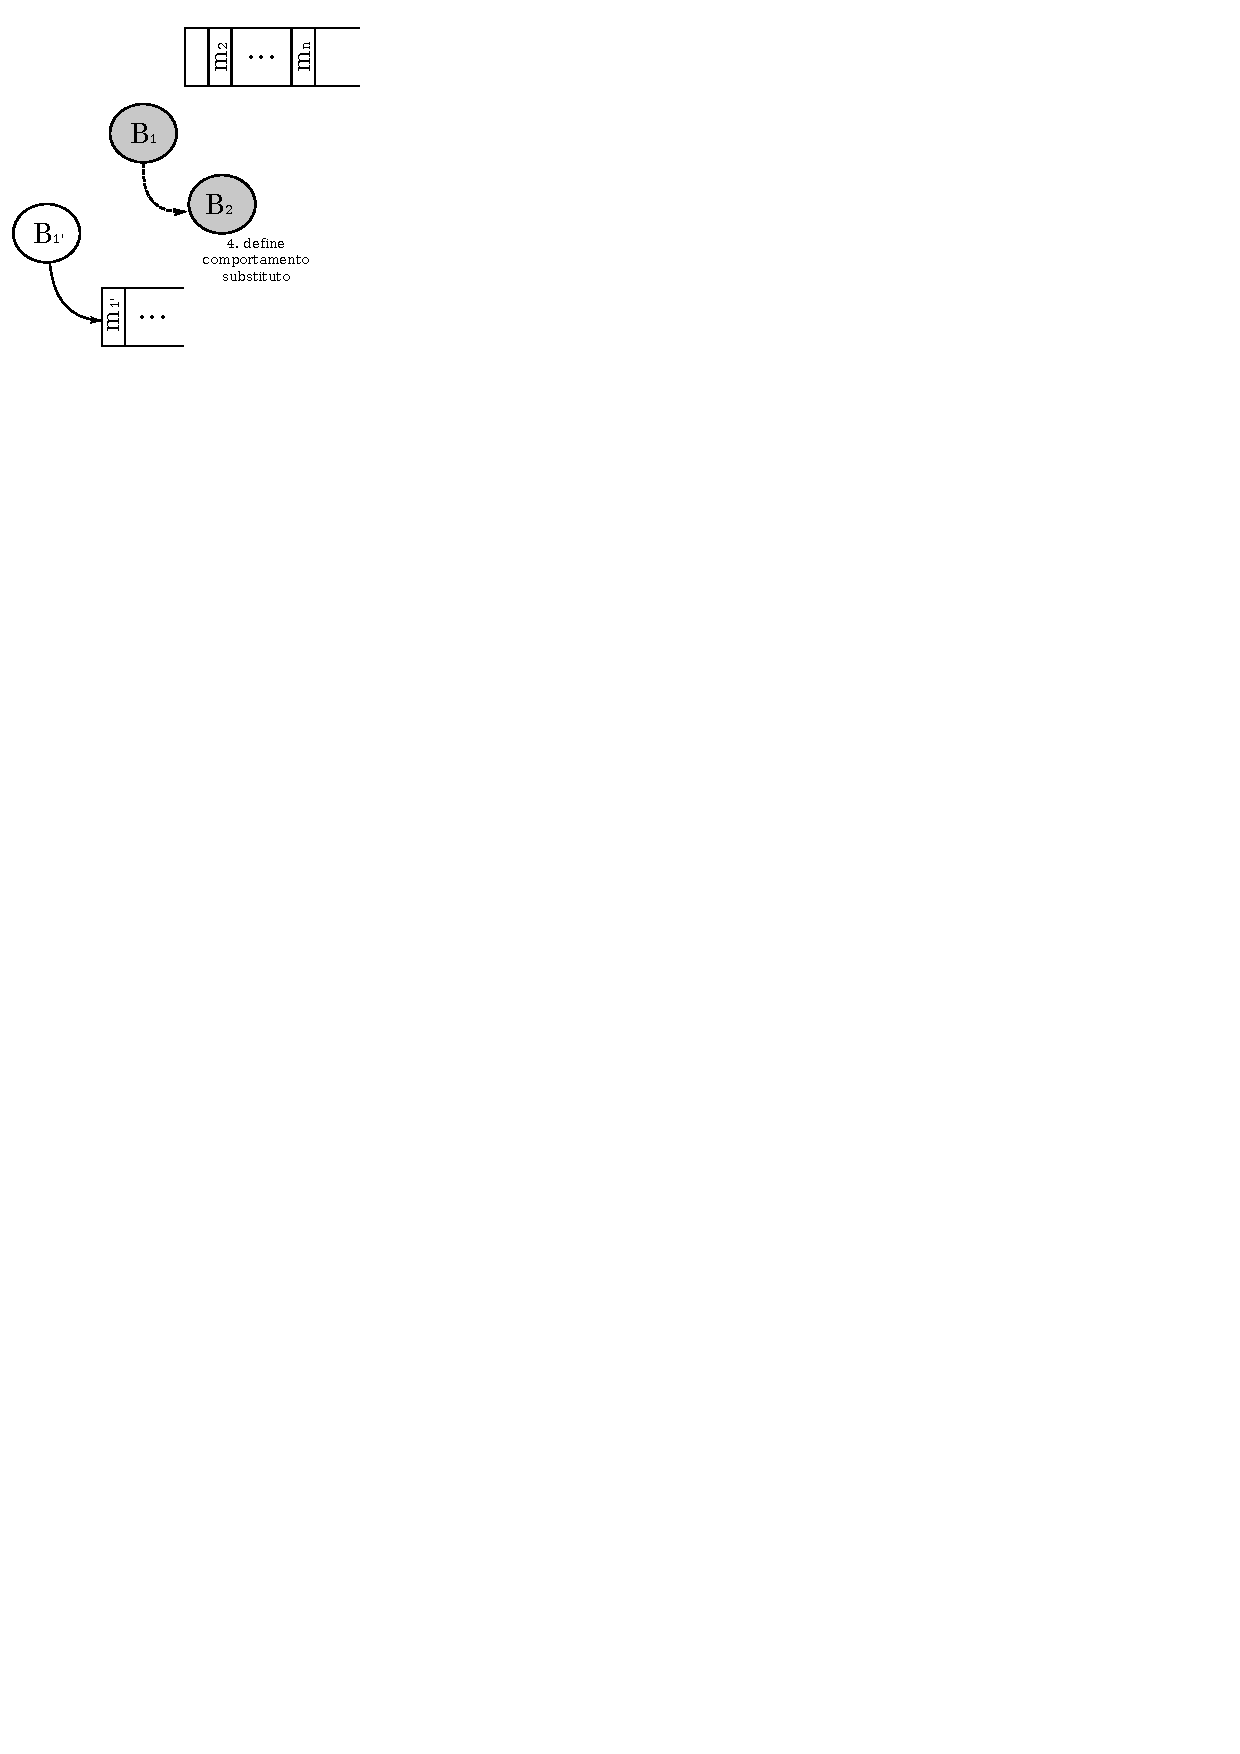
\includegraphics[scale=1.0]{figuras/ator-state-machine4.pdf}
		\end{figure}
	}
	\only<6>{
		\begin{figure}[hbtp]
			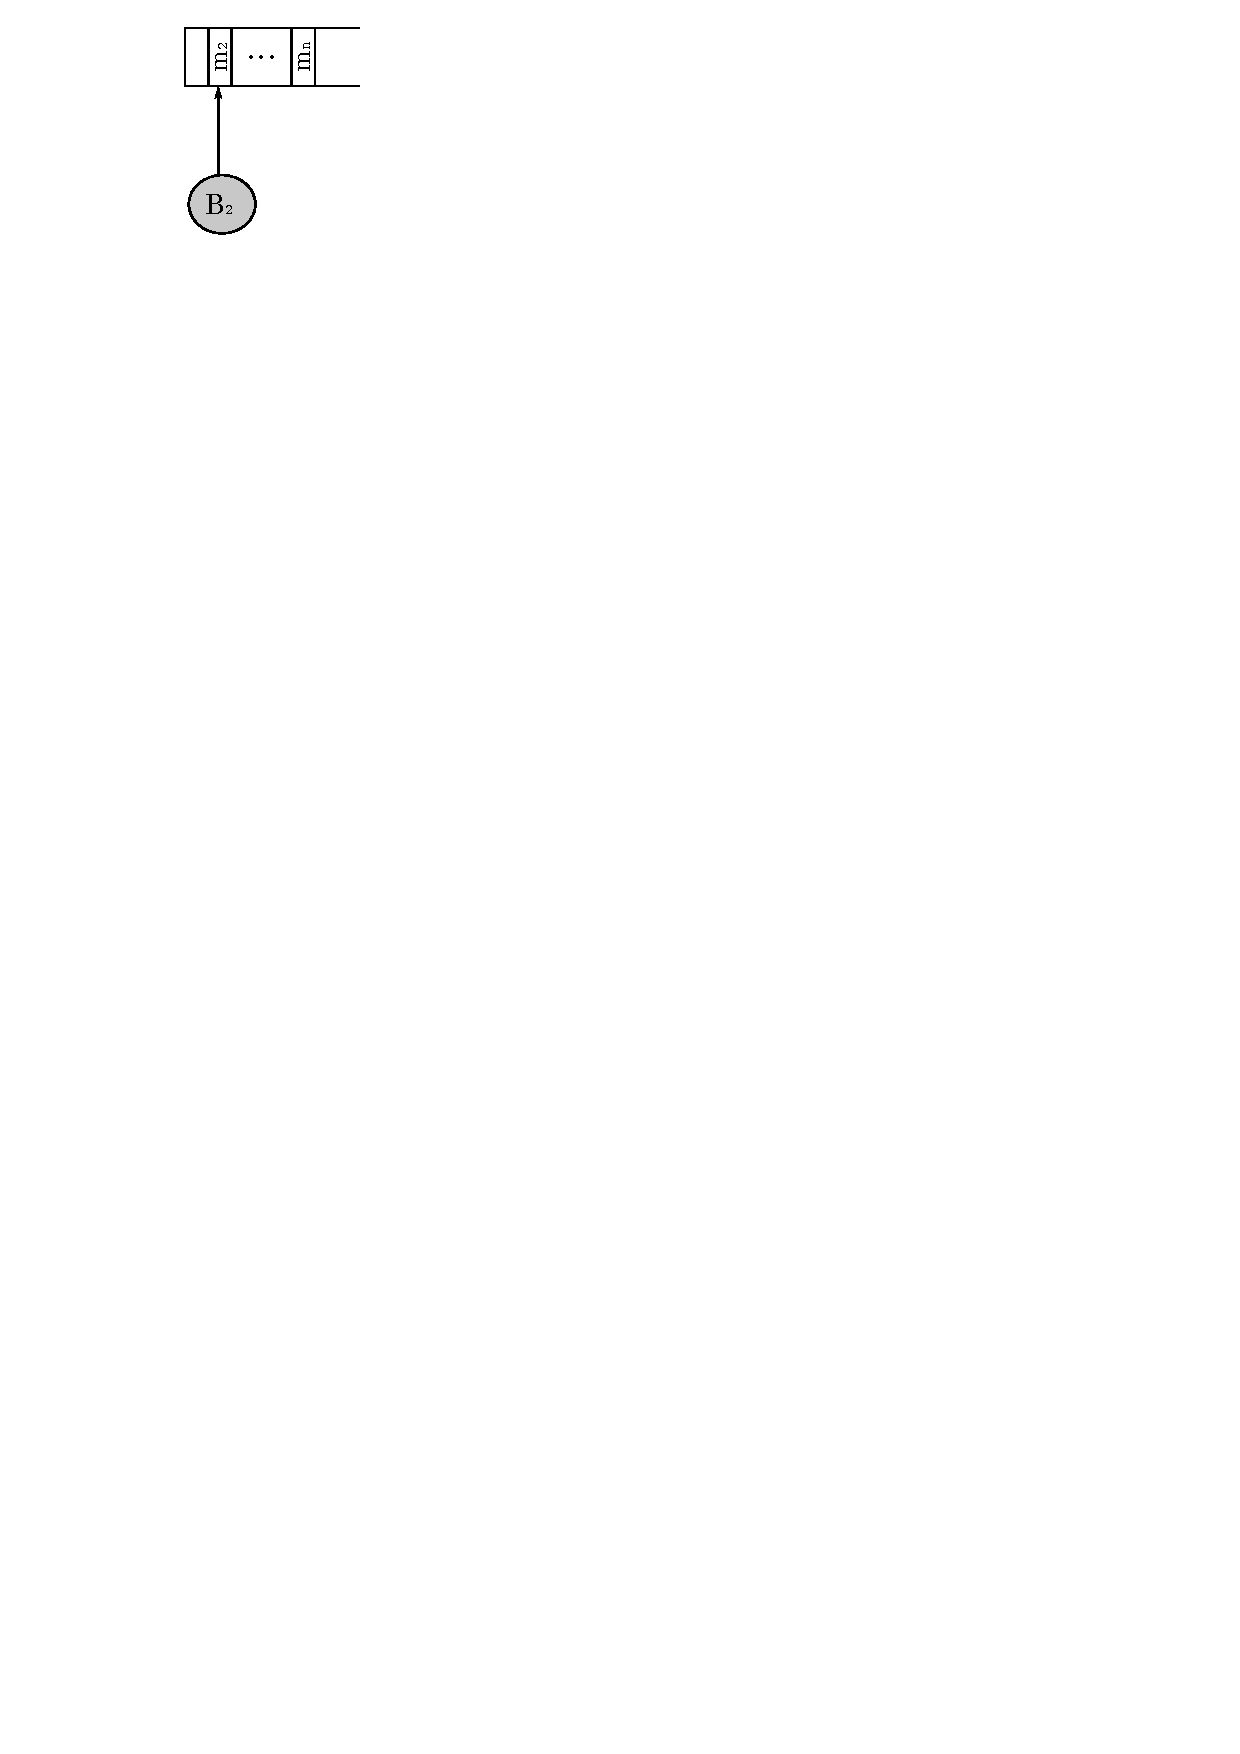
\includegraphics[scale=1.0]{figuras/ator-state-machine5.pdf}
		\end{figure}
	}
	\only<7>{
 		\begin{beamerboxesrounded}{Algumas implementa\c{c}\~oes:}
			\begin{itemize}
				\item Linguagens: Axum, SALSA e Erlang
				\item C++: Act++, Thal e Theron
				\item Smalltalk: Actalk
				\item Python: Parley e Stackless Python
				\item Ruby: Stage e Rubinius
				\item .Net: Asynchronous Agent Library e Retlang
				\item Java: Akka, Kilim, Jetlang e Actor Foundry
				\item Scala: Scala Actors, Akka e Scalaz
			\end{itemize}
		\end{beamerboxesrounded}
 	}
}

\subsection{Advanced Message Queuing Protocol}
\frame{
\frametitle{Advanced Message Queuing Protocol}
	\only<1>{
 		\note{
 			\begin{itemize}
				\item Protocolo aberto desenvolvido por um conjunto de empresas com o objetivo de padroniza\c{c}\~ao
			          e redu\c{c}\~ao de custos na integra\c{c}\~ao de sistemas
				\item Al\'em da defini\c{c}\~ao do protocolo, define tamb\'em a sem\^antica dos servi\c{c}os de trocas de mensagens 
				\item Objetiva que as capacidades de MOMs estejam dispon\'iveis pervasivamente nas empresas
			\end{itemize}
		}
		\begin{figure}[hbtp]
			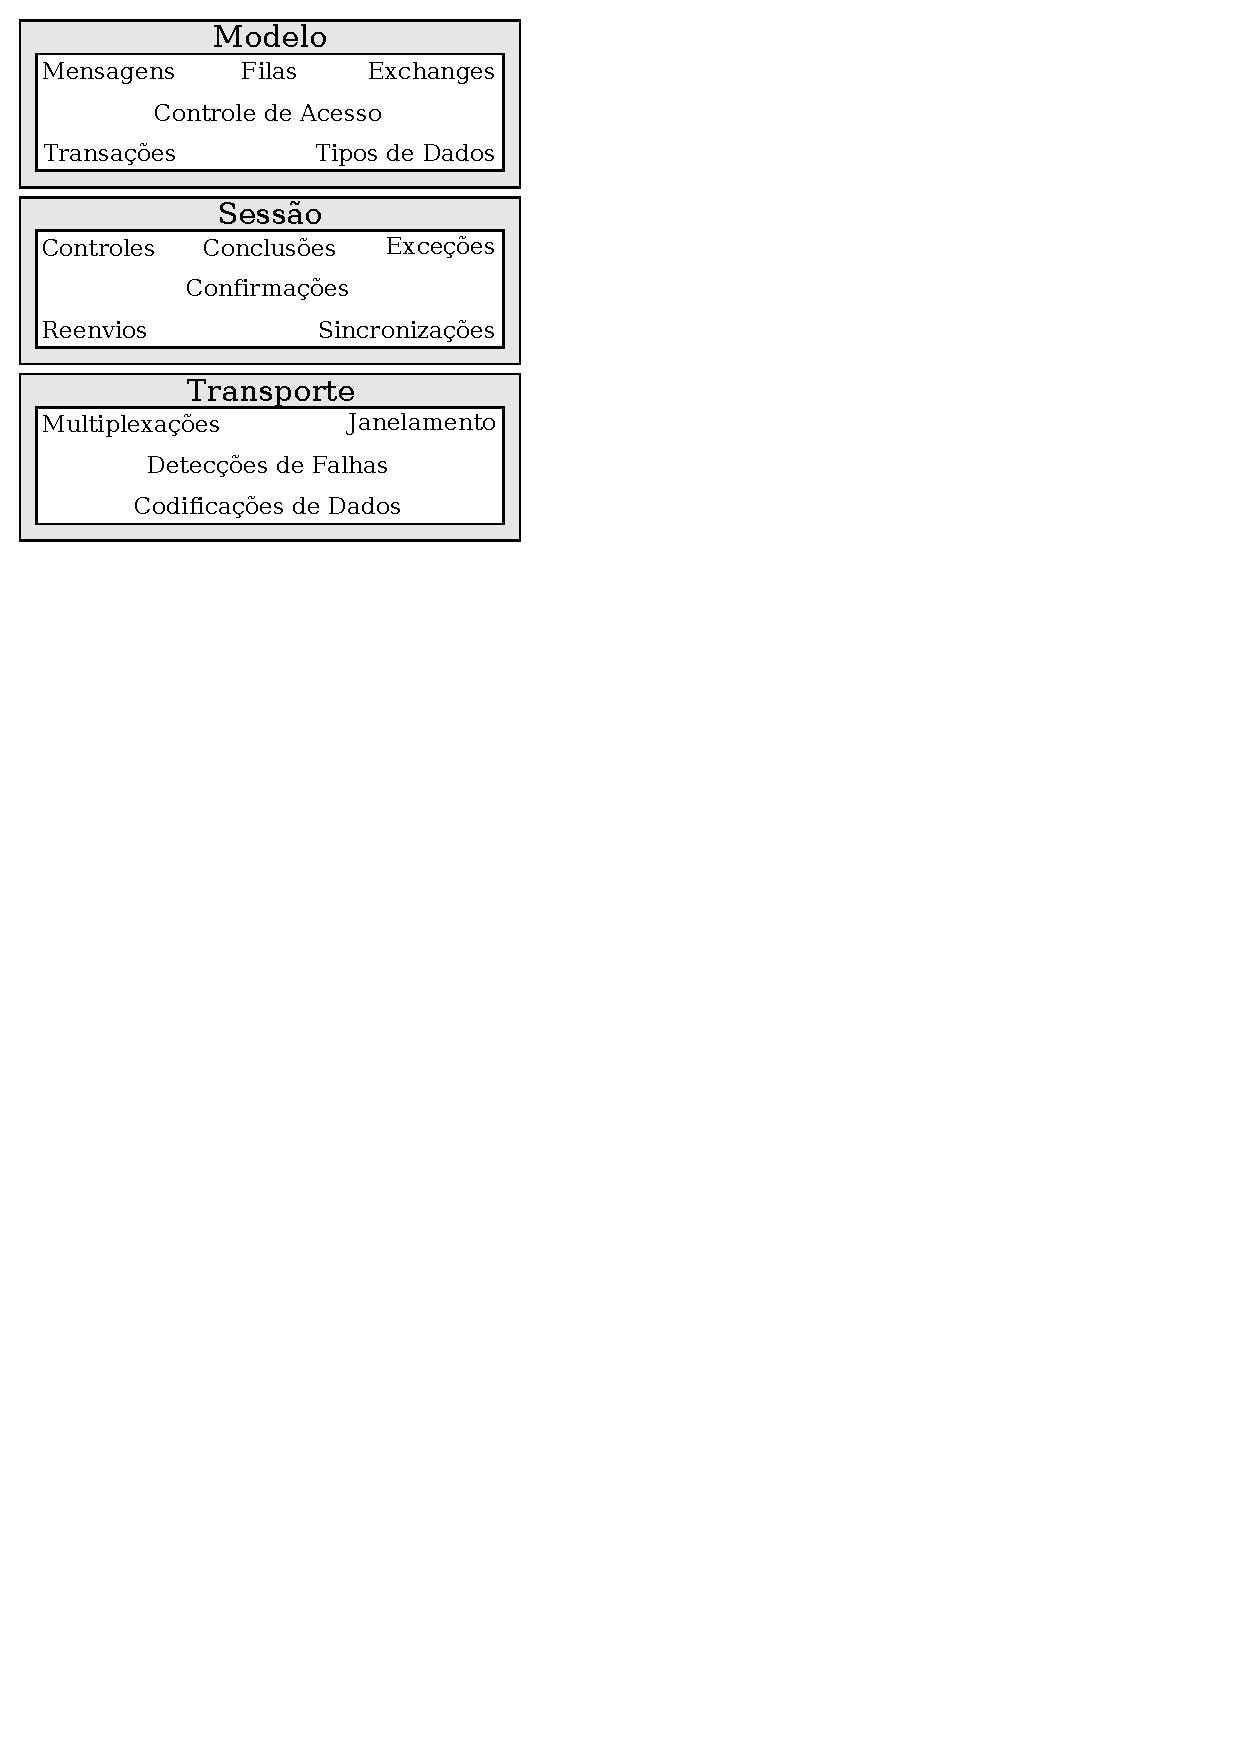
\includegraphics[scale=.60]{figuras/protocol_overview.pdf}
		\end{figure}
	}
	\only<2>{
 		\note{
 			Para nao esquecer: comentar brevemente quem eh quem antes (adicionar outras notas) 					
 		}
		\begin{figure}[hbtp]
			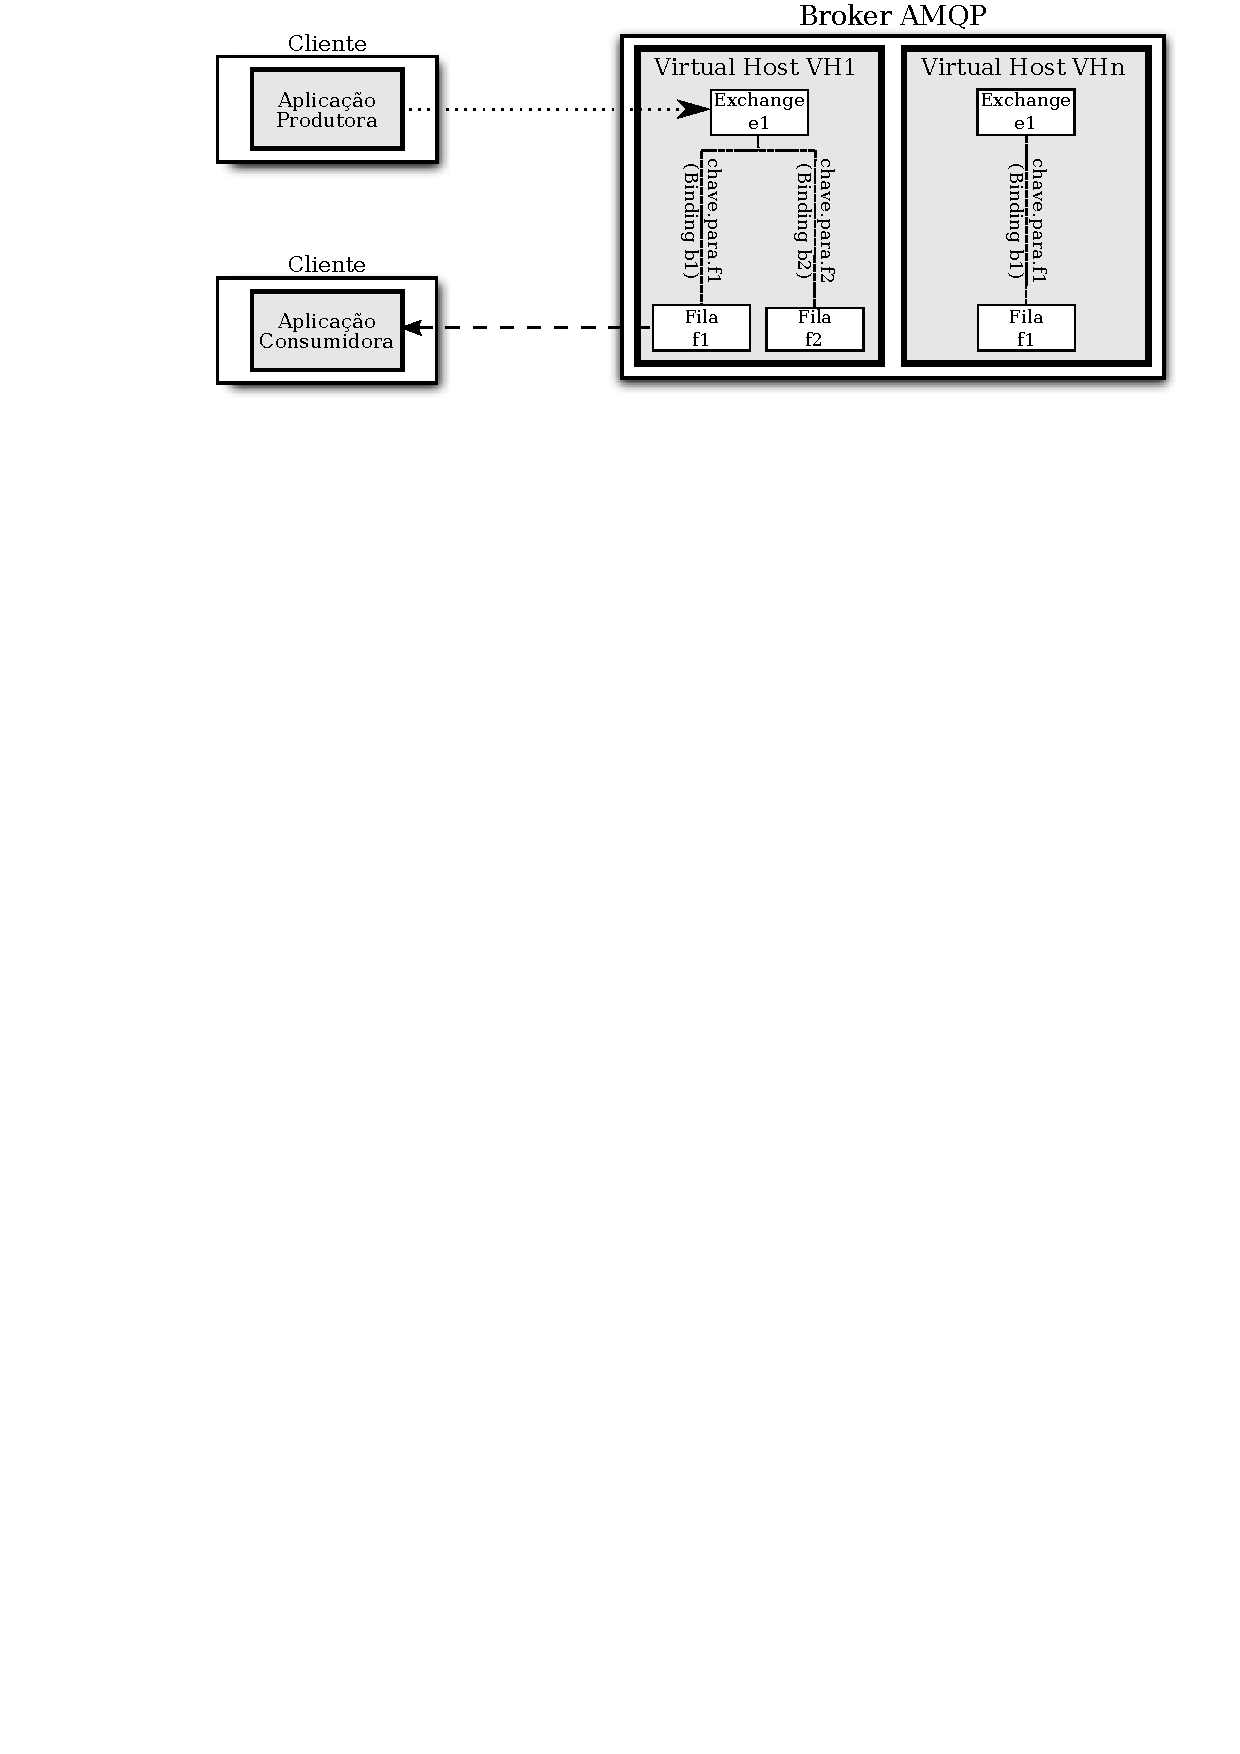
\includegraphics[scale=.70]{figuras/amqp-overview.pdf}
		\end{figure}
	}
 	\only<3>{ 		
  		\begin{figure}[hbtp]
			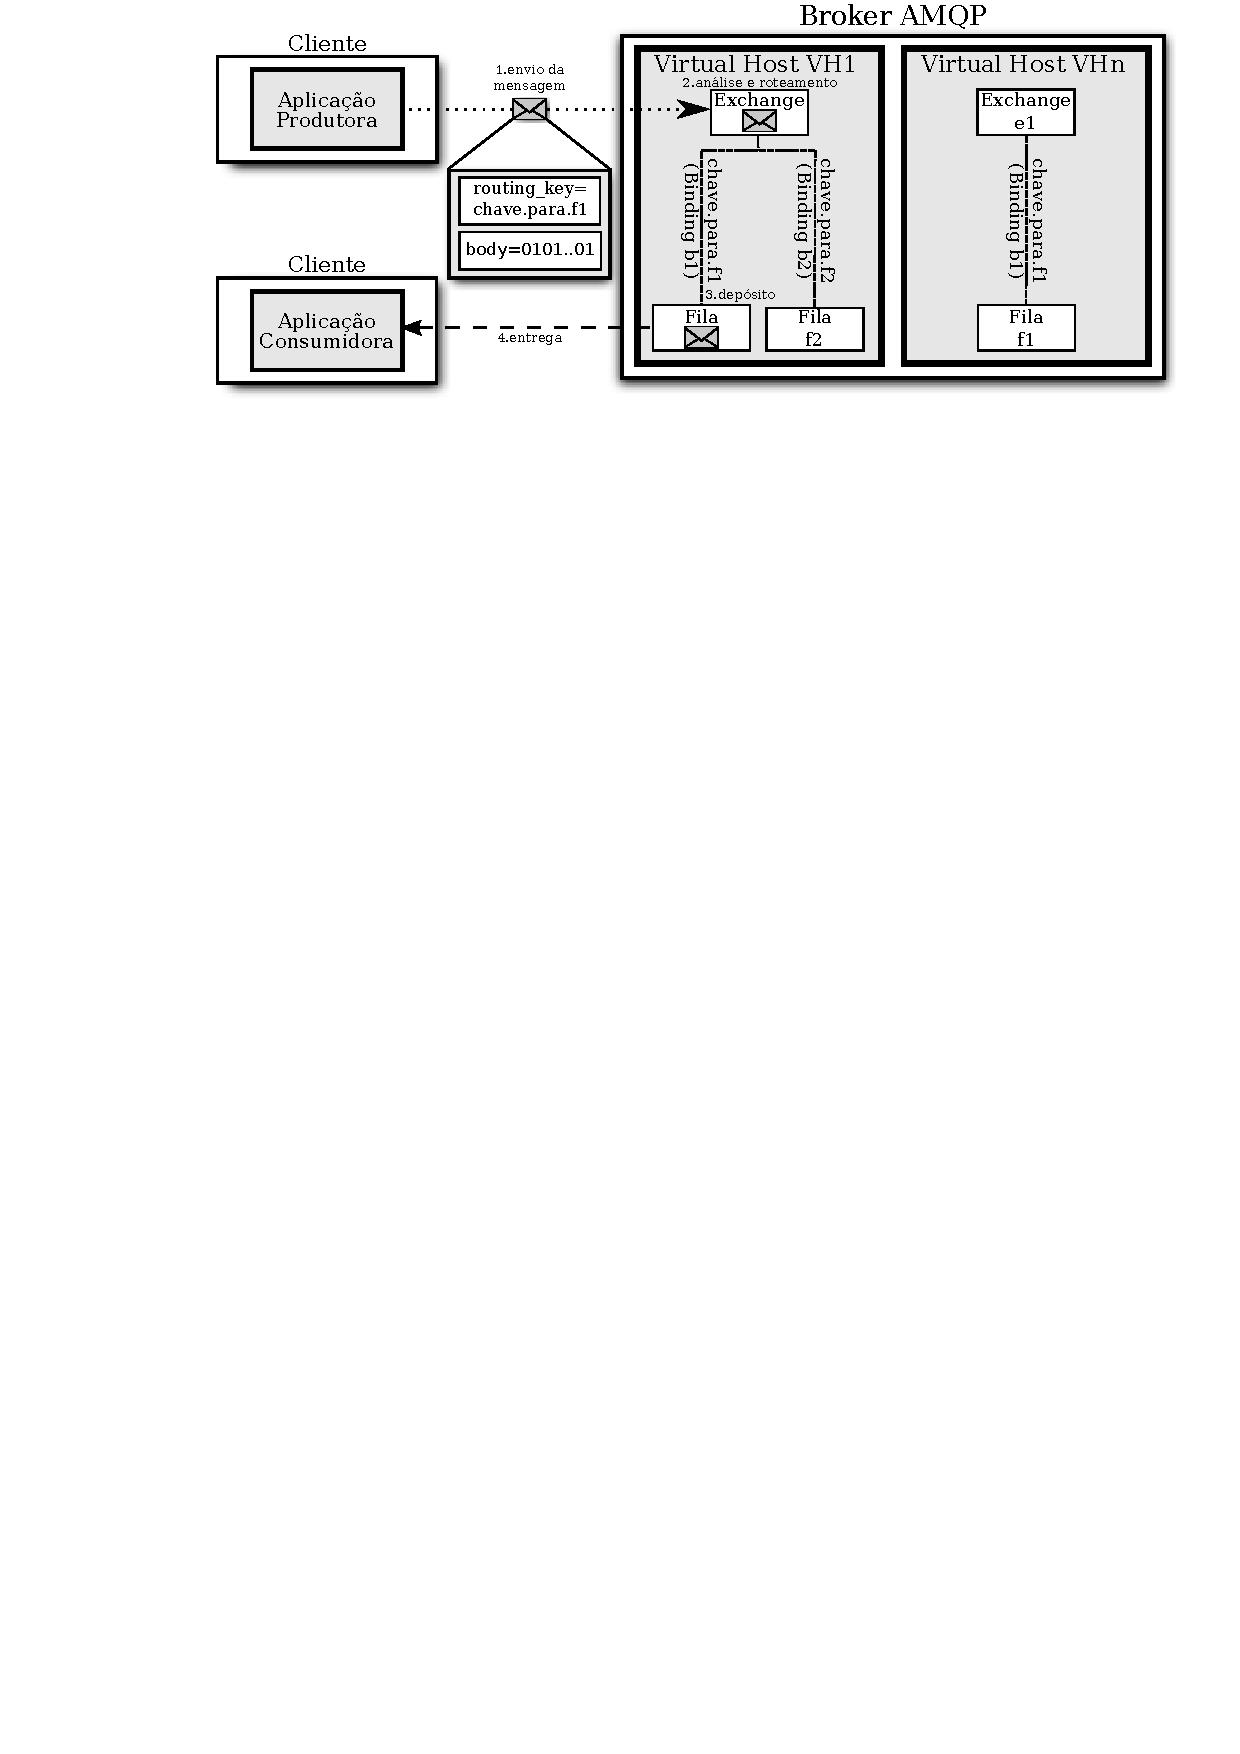
\includegraphics[scale=.70]{figuras/amqp-message-flow.pdf}
		\end{figure}
 	}
	\only<4>{
 		\begin{beamerboxesrounded}{Analogia com sistemas de \textit{email}:}
	 		\begin{itemize}
				\item Mensagens AMQP s\~ao an\'alogas a mensagens de correio eletr\^onico
				\item Filas s\~ao an\'alogas a caixas de correio
				\item \textit{Exchanges} s\~ao an\'alogas a agentes de transfer\^encia de mensagens (MTA).
				 Com base nas chaves de roteamento (To, Cc e Bcc no caso de correio eletr\^onico), eles verificam
				as tabelas de registro e decidem como enviar as mensagens para uma ou mais caixas de correio
				\item \textit{Bindings} correspondem a entradas nas tabelas de roteamento do MTA		
			\end{itemize}
 		\end{beamerboxesrounded}
 	}
}


\frame{
 	\frametitle{Perguntas}
		\begin{figure}[hbtp]
			
\includegraphics[scale=0.5]{figuras/question.pdf}
		\end{figure}
 	}


\end{document}
